\documentclass[12pt,pdf,hyperref={unicode}]{beamer}
%\usetheme{boxes}
\beamertemplatenavigationsymbolsempty
\setbeamertemplate{footline}[page number]
% Set it for the internal PhD thesis defence to reduce number of slides
%\setbeamersize{text margin left=0.5em, text margin right=0.5em}

\usepackage[utf8]{inputenc}
%\usepackage[english, russian]{babel}
\usepackage{bm}
\usepackage{multirow}
\usepackage{ragged2e}
\usepackage{indentfirst}
\usepackage{multicol}
\usepackage{subfig}
\usepackage{amsmath,amssymb}
\usepackage{enumerate}
\usepackage{mathtools}
\usepackage{comment}
\usepackage[all]{xy}
\usepackage{tikz}
\usetikzlibrary{positioning,arrows}
\tikzstyle{name} = [parameters]
\definecolor{name}{rgb}{0.5,0.5,0.5}

%\usepackage{caption}
%\captionsetup{skip=0pt,belowskip=0pt}

%\newtheorem{theorem}{Theorem}
%\newtheorem{statement}{Statement}
%\newtheorem{definition}{Definition}

% colors
\definecolor{darkgreen}{rgb}{0.0, 0.2, 0.13}
\definecolor{darkcyan}{rgb}{0.0, 0.55, 0.55}
%\AtBeginEnvironment{figure}{\setcounter{subfigure}{0}}
%\captionsetup[subfloat]{labelformat=empty}

%----------------------------------------------------------------------------------------------------------

\title{ Evaluating Estimated Depth for Robotic Manipulation: Comparing Monocular and Stereodepth with 3D-LOTUS++}
\author{Kazybek Askarbek}
\institute[HSE]{}
\date{2024}

%---------------------------------------------------------------------------------------------------------
\begin{document}
%\begin{frame}
\titlepage
%\end{frame}
% \setcounter{page}{2}%remove here for the title
%----------------------------------------------------------------------------------------------------------
%\section{Please do not use sectioning in the presentations}
\begin{frame}{}
High-quality depth sensors are costly and noisy. Estimated depth models provide a cheaper, promising alternative for robotic manipulation.
\begin{block}{The problem}
To investigate the feasibility of replacing expensive depth sensors with estimated depth models for robotic manipulation.
\end{block}
\begin{block}{The method needs a proper name here}
We compare different depth sources (sensor, monocular, stereo) as inputs to the 3D-LOTUS++ model, testing manipulation performance, noise robustness, and generalization.
\end{block}
\begin{block}{The solution} 
\begin{enumerate}[1)]
\item Set up a systematic comparison of estimated vs. sensor depth,
\item Put mixed training in place to reduce noise sensitivity,
\item Get a robust, cost-effective solution for depth sensing.
\end{enumerate}
\end{block}
\end{frame}
%----------------------------------------------------------------------------------------------------------
\begin{frame}{Graphical highlights  as a form of your message%
\footnote{\textit{Garcia, Ricardo et al.} "Towards Generalizable Vision-Language Robotic Manipulation: A Benchmark and LLM-guided 3D Policy." (2024).}}
\begin{columns}
\begin{column}{0.3\textwidth}
\begin{enumerate}[1)]
    \item Architecture of SoTA 3D-LOTUS++ model 
\end{enumerate}
\end{column}
\begin{column}{0.7\textwidth}
	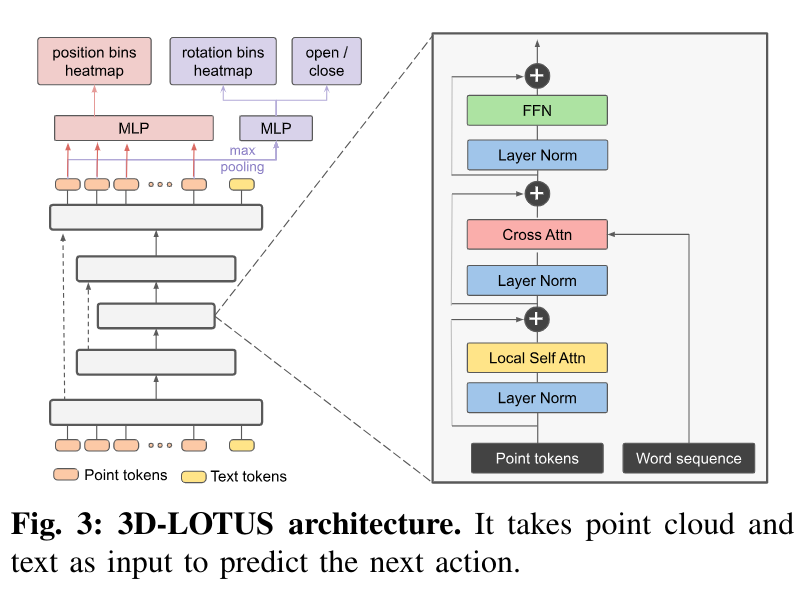
\includegraphics[width=1\textwidth]{3dlotus_arch.png}
\end{column}
\end{columns}
\end{frame}
\end{document}